\chapter{Command模式}
\section{命令模式的概念}
\subsection{定义}
命令(Command)模式的定义如下:将一个请求封装为一个对象,使发出请求的责任和执行请求的责任分割开。这样两者之间通过命令对象进行沟通,这样方便将命令对象进行储存、传递、调用、增加与管理。
\subsection{优点}
\begin{enumerate}
	\item 降低系统的耦合度。命令模式能将调用操作的对象与实现该操作的对象解耦。
	\item 增加或删除命令非常方便。采用命令模式增加与删除命令不会影响其他类,它满足“开闭原则”,对扩展比较灵活。
	\item 可以实现宏命令。命令模式可以与组合模式结合,将多个命令装配成一个组合命令,即宏命令。
	\item 方便实现 Undo 和 Redo 操作。命令模式可以与后面介绍的备忘录模式结合,实现命令的撤销与恢复。
\end{enumerate}
\subsection{缺点}
可能产生大量具体命令类。因为计对每一个具体操作都需要设计一个具体命令类,这将增加系统的复杂性。
\subsection{命令模式的角色}
\begin{enumerate}
	\item Command命令:声明执行命令的接口,拥有执行命令的抽象方法 execute();
	\item ConcreteCommand具体命令:是抽象命令类的具体实现类,它拥有接收者对象,并通过调用接收者的功能来完成命令要执行的操作;
	\item Receiver接收者:执行命令功能的相关操作,是具体命令对象业务的真正实现者。
	\item Client请求者:负责生成ConcreteCommand角色并分配Receiver角色。
	\item Invoker发动者:是请求的发送者,它通常拥有很多的命令对象,并通过访问命令对象来执行相关请求,它不直接访问接收者,调用Command的execute()。
\end{enumerate}
\subsection{应用场景}
\begin{enumerate}
	\item 当系统需要将请求调用者与请求接收者解耦时,命令模式使得调用者和接收者不直接交互。
	\item 当系统需要随机请求命令或经常增加或删除命令时,命令模式比较方便实现这些功能。
	\item 当系统需要执行一组操作时,命令模式可以定义宏命令来实现该功能。
	\item 当系统需要支持命令的撤销(Undo)操作和恢复(Redo)操作时,可以将命令对象存储起来,采用备忘录模式来实现。
\end{enumerate}
\section{命令模式实现——例一}
\begin{figure}[!h]
	\centering
	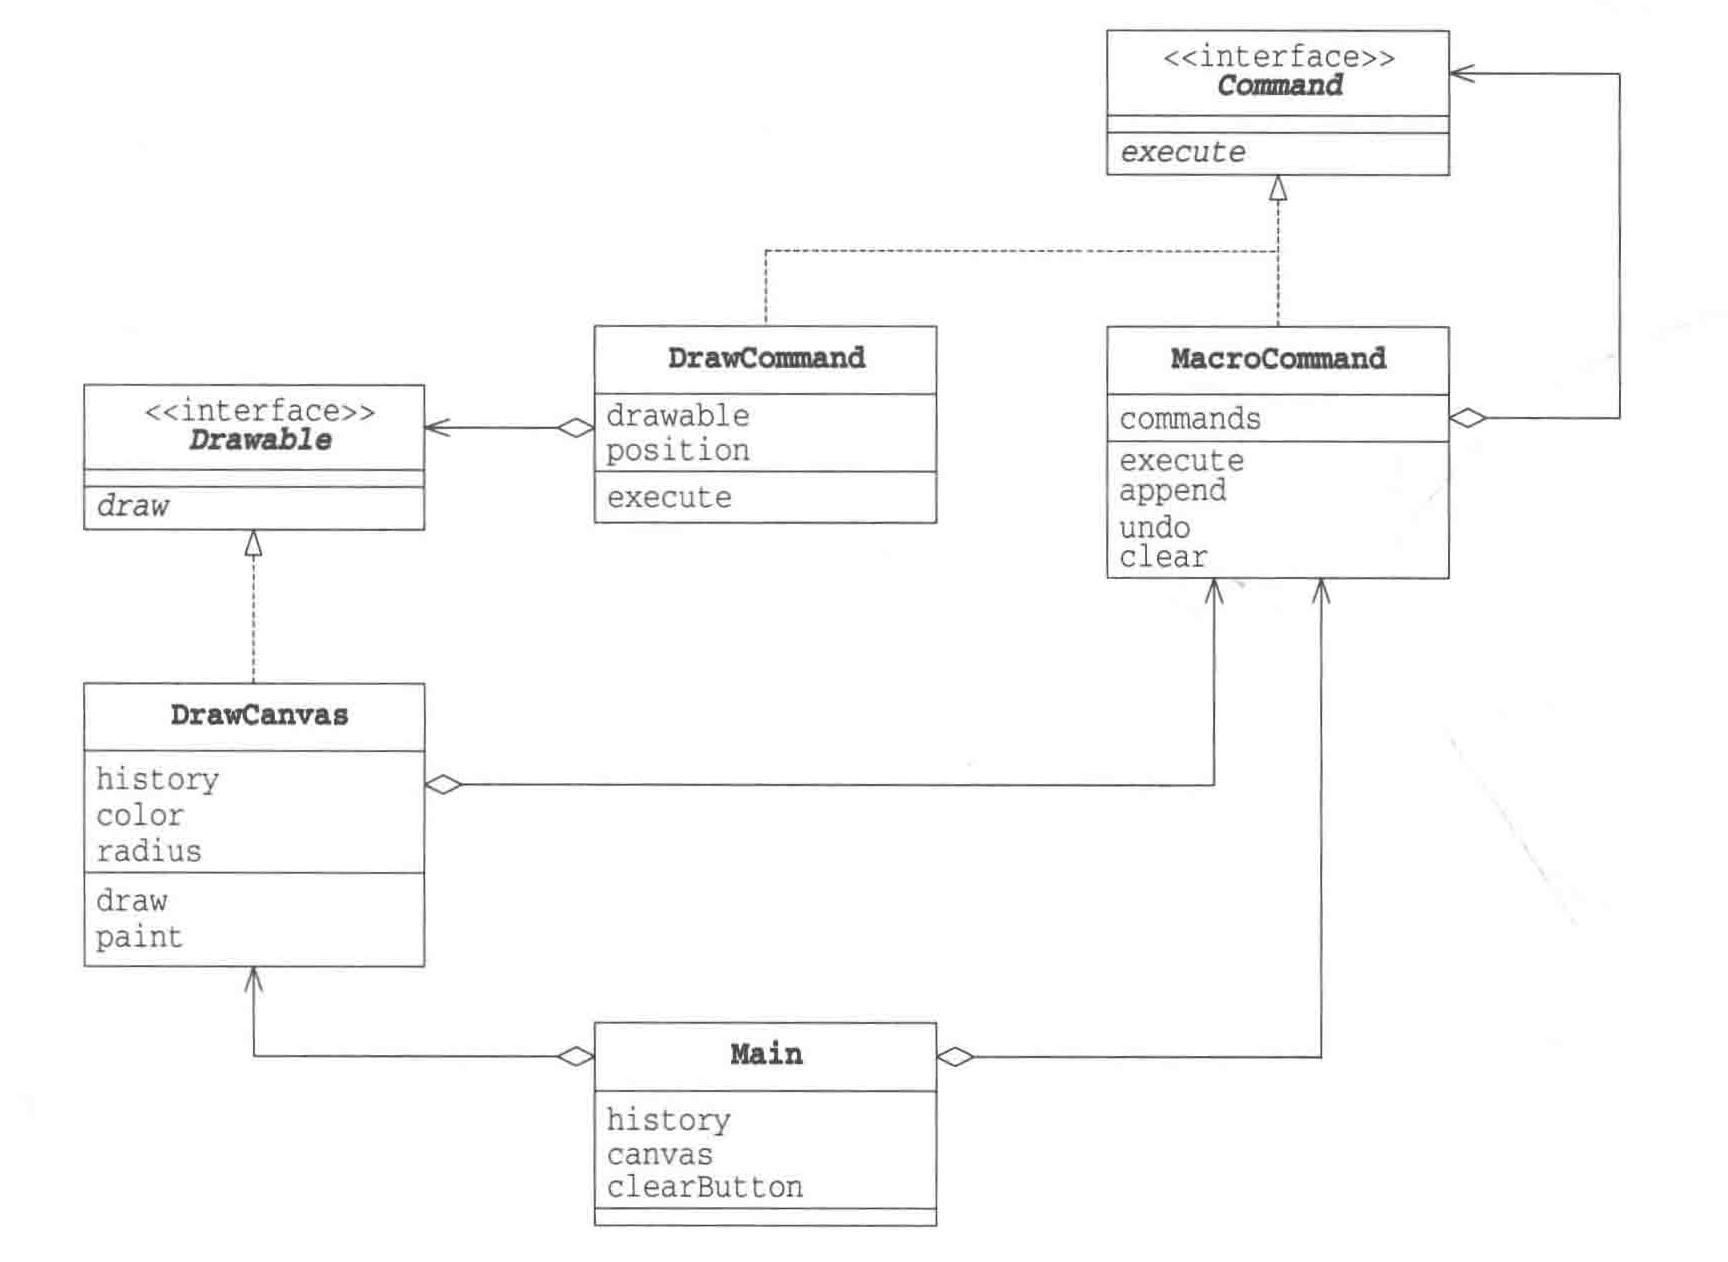
\includegraphics[width=\textwidth]{image/22-1}
	\caption{命令模式的类图}
\end{figure}
\begin{lstlisting}
// Command 角色,只需要定义一个方法
public interface Command {
	void execute();
}
\end{lstlisting}
\begin{lstlisting}
// 表示绘制对象的接口,也是 Receiver 角色
public interface Drawable {
	void draw(int x, int y);
}
\end{lstlisting}
\begin{lstlisting}
// 绘制一个点的命令
public class DrawCommand implements Command {
	// 绘制对象
	protected Drawable drawable;
	//绘制位置
	private Point position;
	
	public DrawCommand(Drawable drawable, Point position) {
		this.drawable = drawable;
		this.position = position;
	}
	public void execute() {
		drawable.draw(position.x, position.y);
	}
}
\end{lstlisting}
\begin{lstlisting}
// 画板
public class DrawCanvas extends Canvas implements Drawable {
	private Color color = Color.red;
	private int radius = 6;
	//命令的历史记录
	private MacroCommand history;
	
	public DrawCanvas(int width, int height, MacroCommand history) {
		setSize(width, height);
		setBackground(Color.white);
		this.history = history;
	}
	
	// 全部重新绘制
	public void paint(Graphics graphics) {
		history.execute();
	}
	
	public void draw(int x, int y) {
		Graphics graphics = getGraphics();
		graphics.setColor(color);
		graphics.fillOval(x - radius, y - radius, radius * 2, radius * 2);
	}
}
\end{lstlisting}
\begin{lstlisting}
//由多条命令整合的命令
public class MacroCommand implements Command {
	//命令的集合
	private Stack<Command> commands = new Stack<>();
	
	public void execute() {
		Iterator<Command> it = commands.iterator();
		while (it.hasNext()) {
			it.next().execute();
		}
	}
	
	//添加命令
	public void append(Command command) {
		if (command != this) {
			commands.push(command);
		}
	}
	
	//删除最后一条命令,达到撤销命令的目的
	public void undo() {
		if (!commands.empty()) {
			commands.pop();
		}
	}
	
	//删除所有命令
	public void clear() {
		commands.clear();
	}
}
\end{lstlisting}
\begin{lstlisting}
public class Main extends JFrame implements ActionListener, MouseMotionListener, WindowListener {
	//绘制的历史记录
	private MacroCommand history = new MacroCommand();
	//绘制区域
	private DrawCanvas canvas = new DrawCanvas(400, 400, history);
	//删除按钮
	private JButton clearButton = new JButton("clear");
	
	public Main(String title) throws HeadlessException {
		super(title);
		this.addWindowListener(this);
		canvas.addMouseMotionListener(this);
		clearButton.addActionListener(this);
		
		Box buttonBox = new Box(BoxLayout.X_AXIS);
		buttonBox.add(clearButton);
		Box mainBox = new Box(BoxLayout.Y_AXIS);
		mainBox.add(buttonBox);
		mainBox.add(canvas);
		getContentPane().add(mainBox);
		pack();
		show();
	}
	
	public static void main(String[] args) {
		new Main("Command Pattern Sample");
	}
	
	public void actionPerformed(ActionEvent e) {
		if (e.getSource() == clearButton) {
			history.clear();
			canvas.repaint();
		}
	}
	
	public void mouseDragged(MouseEvent e) {
		Command cmd = new DrawCommand(canvas, e.getPoint());
		history.append(cmd);
		cmd.execute();
	}
	
	public void mouseMoved(MouseEvent e) {}
	
	public void windowOpened(WindowEvent e) {}
	
	public void windowClosing(WindowEvent e) {
		System.exit(0);
	}
	
	public void windowClosed(WindowEvent e) {}
	
	public void windowIconified(WindowEvent e) {}
	
	public void windowDeiconified(WindowEvent e) {}
	
	public void windowActivated(WindowEvent e) {}
	
	public void windowDeactivated(WindowEvent e) {}
}
\end{lstlisting}
\section{命令模式实现——例二}
\begin{figure}[!h]
	\centering
	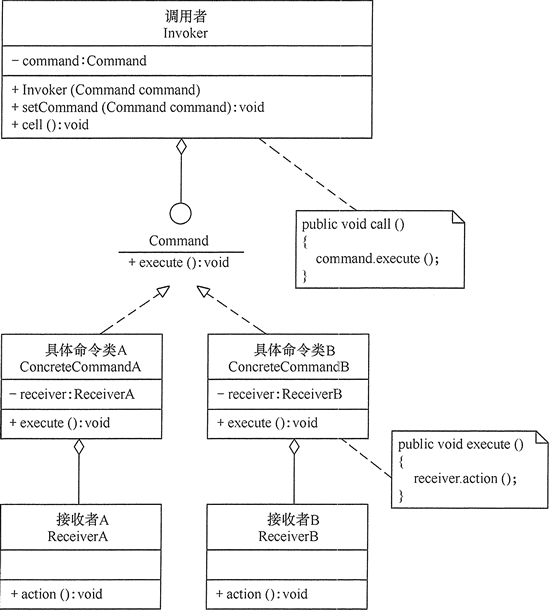
\includegraphics[width=0.6\textwidth]{image/22-2}
	\caption{命令模式的结构图}
\end{figure}
\begin{lstlisting}
//抽象命令
interface Command {
	public abstract void execute();
}

//具体命令
class ConcreteCommand implements Command {
	private Receiver receiver;
	
	ConcreteCommand() {
		receiver = new Receiver();
	}
	
	public void execute() {
		receiver.action();
	}
}
\end{lstlisting}
\begin{lstlisting}
//接收者
class Receiver {
	public void action() {
		System.out.println("接收者的action()方法被调用...");
	}
}
\end{lstlisting}
\begin{lstlisting}
//调用者
class Invoker {
	private Command command;
	
	public Invoker(Command command) {
		this.command = command;
	}
	
	public void setCommand(Command command) {
		this.command = command;
	}
	
	public void call() {
		System.out.println("调用者执行命令command...");
		command.execute();
	}
}
\end{lstlisting}
\begin{lstlisting}
public class CommandPattern {
	public static void main(String[] args) {
		Command cmd = new ConcreteCommand();
		Invoker ir = new Invoker(cmd);
		System.out.println("客户访问调用者的call()方法...");
		ir.call();
	}
}
\end{lstlisting}
\begin{lstlisting}
//output
客户访问调用者的call()方法...
调用者执行命令command...
接收者的action()方法被调用...
\end{lstlisting}
\section{模式扩展}
在软件开发中,有时将命令模式与组合模式联合使用,这就构成了宏命令模式,也叫组合命令模式。宏命令包含了一组命令,它充当了具体命令与调用者的双重角色,执行它时将递归调用它所包含的所有命令。
\begin{figure}[!h]
	\centering
	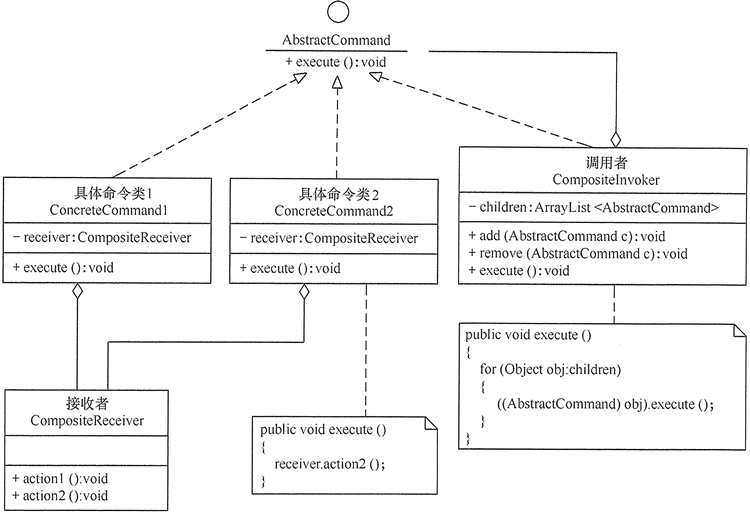
\includegraphics[width=0.8\textwidth]{image/22-3}
	\caption{组合命令模式的结构图}
\end{figure}
\begin{lstlisting}
//抽象命令
interface AbstractCommand {
	public abstract void execute();
}

//树叶构件: 具体命令1
class ConcreteCommand1 implements AbstractCommand {
	private CompositeReceiver receiver;
	
	ConcreteCommand1() {
		receiver = new CompositeReceiver();
	}
	
	public void execute() {
		receiver.action1();
	}
}

//树叶构件: 具体命令2
class ConcreteCommand2 implements AbstractCommand {
	private CompositeReceiver receiver;
	
	ConcreteCommand2() {
		receiver = new CompositeReceiver();
	}
	
	public void execute() {
		receiver.action2();
	}
}
\end{lstlisting}
\begin{lstlisting}
//树枝构件: 调用者
class CompositeInvoker implements AbstractCommand {
	private ArrayList<AbstractCommand> children = new ArrayList<AbstractCommand>();
	
	public void add(AbstractCommand c) {
		children.add(c);
	}
	
	public void remove(AbstractCommand c) {
		children.remove(c);
	}
	
	public AbstractCommand getChild(int i) {
		return children.get(i);
	}
	
	public void execute() {
		for (Object obj : children) {
			((AbstractCommand) obj).execute();
		}
	}
}
\end{lstlisting}
\begin{lstlisting}
//接收者
class CompositeReceiver {
	public void action1() {
		System.out.println("接收者的action1()方法被调用...");
	}
	
	public void action2() {
		System.out.println("接收者的action2()方法被调用...");
	}
}
\end{lstlisting}
\begin{lstlisting}
public class CompositeCommandPattern {
	public static void main(String[] args) {
		AbstractCommand cmd1 = new ConcreteCommand1();
		AbstractCommand cmd2 = new ConcreteCommand2();
		CompositeInvoker ir = new CompositeInvoker();
		ir.add(cmd1);
		ir.add(cmd2);
		System.out.println("客户访问调用者的execute()方法...");
		ir.execute();
	}
}
\end{lstlisting}
\begin{lstlisting}
//output
客户访问调用者的execute()方法...
接收者的action1()方法被调用...
接收者的action2()方法被调用...
\end{lstlisting}
\section{思路扩展}
\begin{enumerate}
	\item 命令中包含信息:ConcreteCommand要知道自己的Receiver角色;
	\item 保存历史记录;
	\item 适配器的结合使用,如例一中使用适配器:
	\begin{lstlisting}
canvas.addMouseMotionListener(new MouseAdapter() {
		public void mouseDragged(MouseEvent e) {
			//execute command
		}
	});
	\end{lstlisting}
\end{enumerate}
\section{相关设计模式}
\begin{enumerate}
	\item Composite模式:使用Composite实现宏命令;
	\item Memento模式:保存Command历史记录;
	\item Protype模式:使用它来复制发生的事情;
\end{enumerate}